\documentclass{article}
\usepackage[margin=1in, paperwidth=8.5in, paperheight=11in]{geometry}
\usepackage{caption}
\usepackage{subcaption}
\usepackage{float}
\usepackage{graphicx}
\usepackage[utf8]{inputenc}
\usepackage{hyperref}

\begin{document}

\setcounter{section}{2}
\setcounter{subsection}{11}
\subsection{Torque Encoder}
\subsubsection{Description/Additional Circuitry}
%Describe your concept of the RTDS, how is the sound produced, what are the parameters for activating the RTDS, etc.
Two rotary potentiometers are mechanically housed in one unit from Active Sensors (P/N MHR5621) and mounted to the rotating shaft of the throttle pedal assembly. The use of a single housing eliminates concerns regarding mechanical backlash and misalignment. Each output from the potentiometers will go to a CAN connected ATmega16M1, which will compare the two outputs and send a message via CAN bus to the motor controllers with the requested torque.
\begin{table}[H]
	    \centering
	        Torque encoder manufacturer and type & MHR5621 from Active Sensors  \\ \hline
	        Torque encoder principle  & Potentiometer \\ \hline
	         Supply Voltage & 5V\\ \hline
	        Minimum Supply Current & 15 mV \\ \hline
	        Operating Temperature & -55 to 150 °C \\ \hline
	        Used Output & 0 - V \\ \hline
	    \end{tabular}
	    \caption{Table 27: Accelerator Pedal Position Sensor data }
	    \label{cells}
	\end{table}
\subsubsection{Torque Encoder Plausibility Check}
Two potentiometers are mounted on the torque pedal. A CAN node probes the voltage dividers which are amplified in different transfer functions using a Texas Instruments Operational Amplifier, part number LMV341QDCKRQ1. One transfer function amplifies the voltage of one potentiometer by a factor of two and the other amplifies the voltage from the potentiometer by a factor of one half. The ATmega will compare the two independent voltages and if an implausibility occurs, a difference in voltage from the Torque Encoder besides what is expected from the transfer function, and persists for more than 100msecc, the power to the motor(s) must be immediately shut down completely. If a short circuit or wiring failure with either potentiometer occurs, the input will be outside the normal operating range, and the power to the motor controllers will be shut down. The node will log the error in the CAN bus. There will also be a Pegasus Brake light pressure switch (part number 3601, recommended by Formula Hybrid) on the brakes, wired to a CAN node with 22 gauge wire. If the pressure switch indicates actuation of the brake and the potentiometers measure more than 25 percent pedal travel, the power to the motors will be completely stopped until the accelerator pedal indicates less than 5 percent pedal travel. 
\subsubsection{Wiring}
%Describe wiring, show schematics, describe connectors and cables and show useful data regarding the wiring.
Two potentiometers are wired with their each input wired through an operational amplifier with a specific amplification, one with an amplification of two and one with an amplification of one half, and their output to the CAN analog input pins. The potentiometers are given separate power lines of 5V, parallel, to the supply power of the CAN node itself. The brake switch is positioned to trip at a level of hard braking, and when triggered will deliver 5V to a CAN input pin. The CAN node is wired to send and receive messages to the other nodes. 


\begin{figure}[h]
	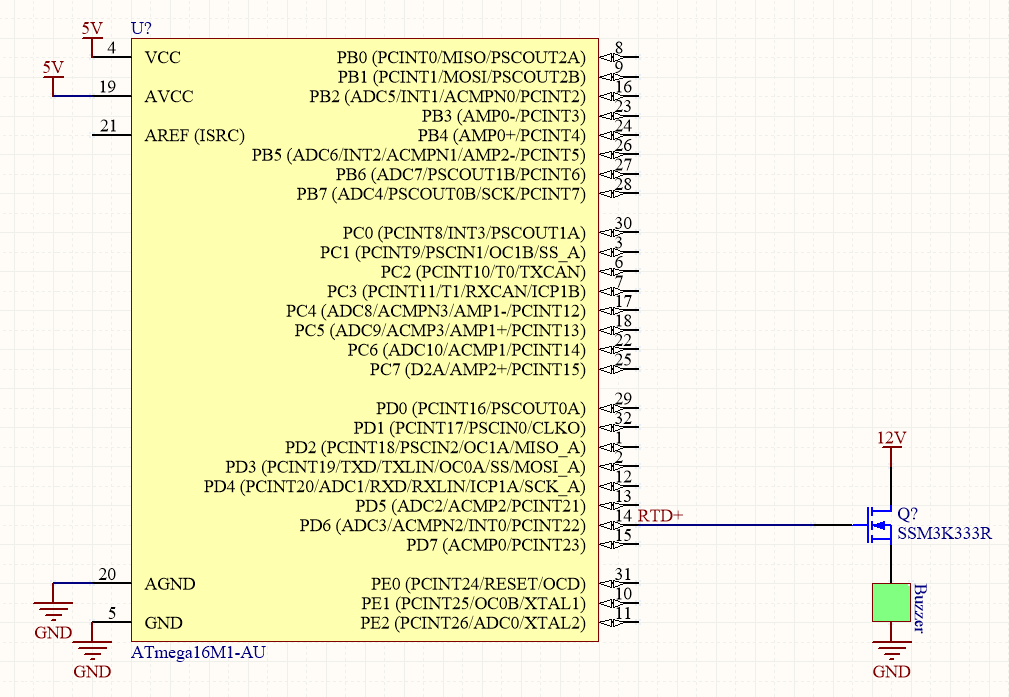
\includegraphics[width=\linewidth]{RTDS_Schematic_Simplified}
	\caption{Torque Encoder Schematic of PCB}
\end{figure}
\begin{figure}[H]
	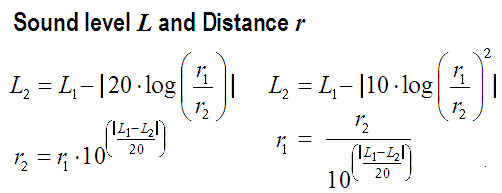
\includegraphics[width=\linewidth]{FormulasForDistanceAndSoundLevel}
	\caption{Inverse Square Law equations needed to calculate the volume at a certain distance}
\end{figure}
Using the inverse square law as referenced in the appendix  for sound pressure levels \ref{Ready to Drive}, 97db at 122cm will translate to 93db at 2m which is a loud enough volume without inducing harm to the listener. 
\subsubsection{Position in Car/Mechanical Connection}
%Provide CAD-renderings showing all relevant parts. Mark the parts in the rendering, if necessary.
The torque encoder is bolted to the accelerator pedal assembly with 4x ¼”-20 bolts. The bolts are safetywired to prevent loosening. The torque encoder is manufactured with a D-shaft. This is rotationally fixed to the accelerator pedal axle by a 4-40 set screw. The set screw is bonded with Loctite Purple to prevent loosening. This allows the torque encoder to measure the angular position of the accelerator pedal axle. The accelerator pedal axle is prevented from moving axially by retaining rings. The mounting of the torque encoder does not affect the relative plausibility check. The sensor used contains two independent encoders, each measuring the position of the single shaft 

\newpage
\setcounter{section}{10}
\section{Appendix}
\setcounter{subsection}{11}
\subsection{Ready to Drive Sound}\label{Ready to Drive}
	\begin{figure}[H]
        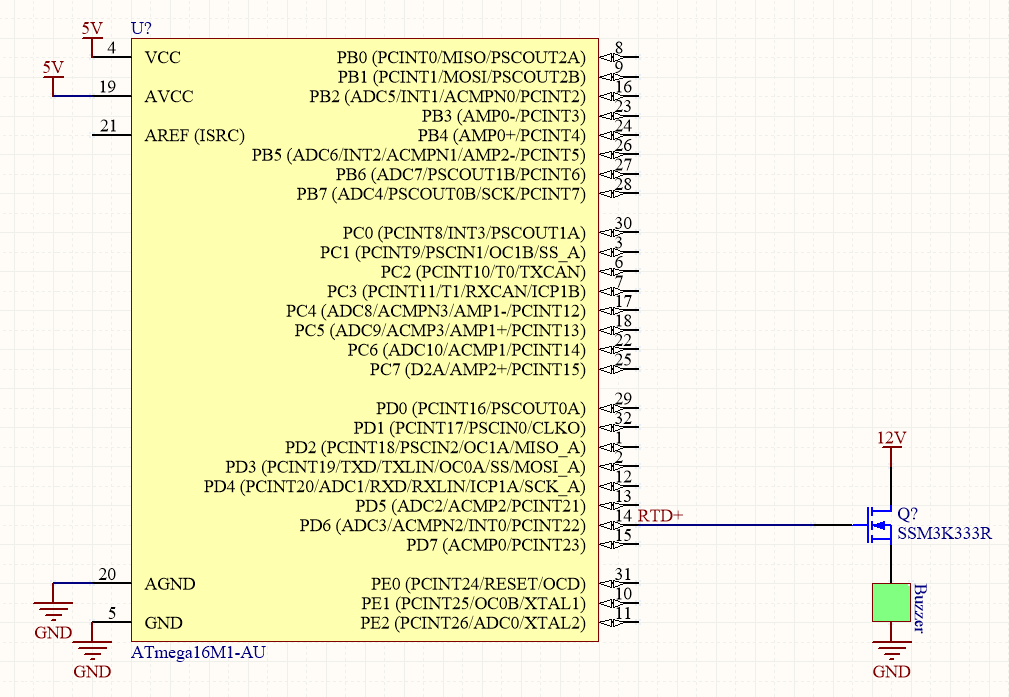
\includegraphics[width=\linewidth]{RTDS_Schematic_Simplified}
        \caption{Ready to Drive Sound Schematic as a subsystem of the dashboard's PCB}
\end{figure}

Ready to drive buzzer \href{http://www.mallory-sonalert.com/specifications/STA20502.PDF}{datasheet}. \newline
\begin{figure}[H]
	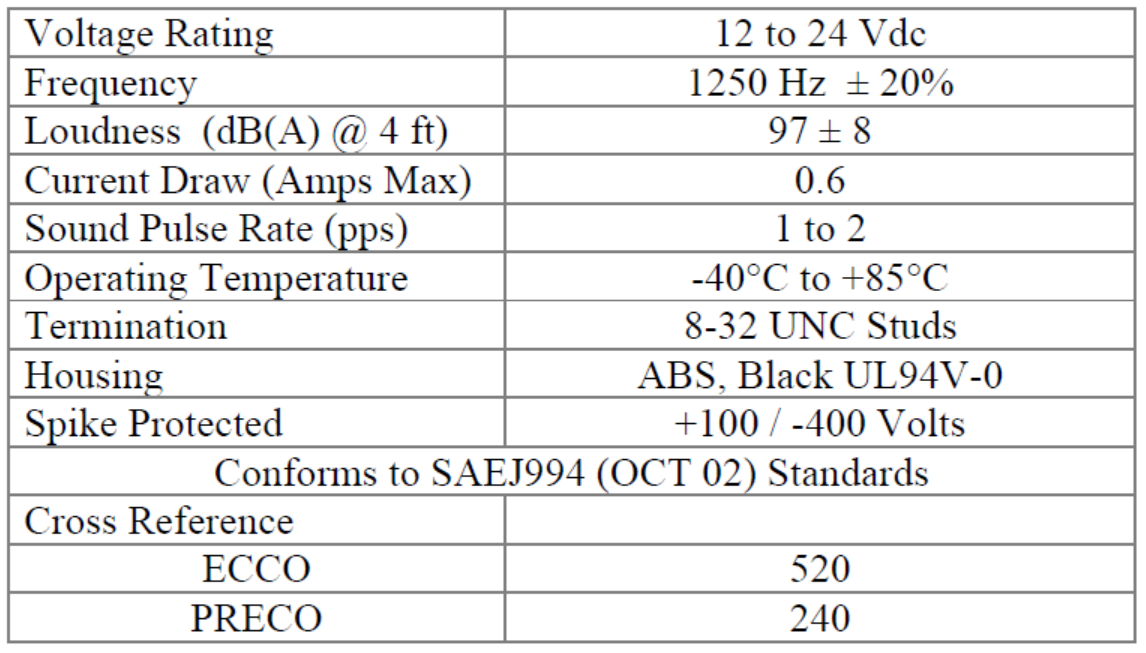
\includegraphics[width=\linewidth]{Buzzer_Specifications}
	\caption{Specification for Mallory Sonalert STA20502 Buzzer}
\end{figure}

\begin{figure}[H]
	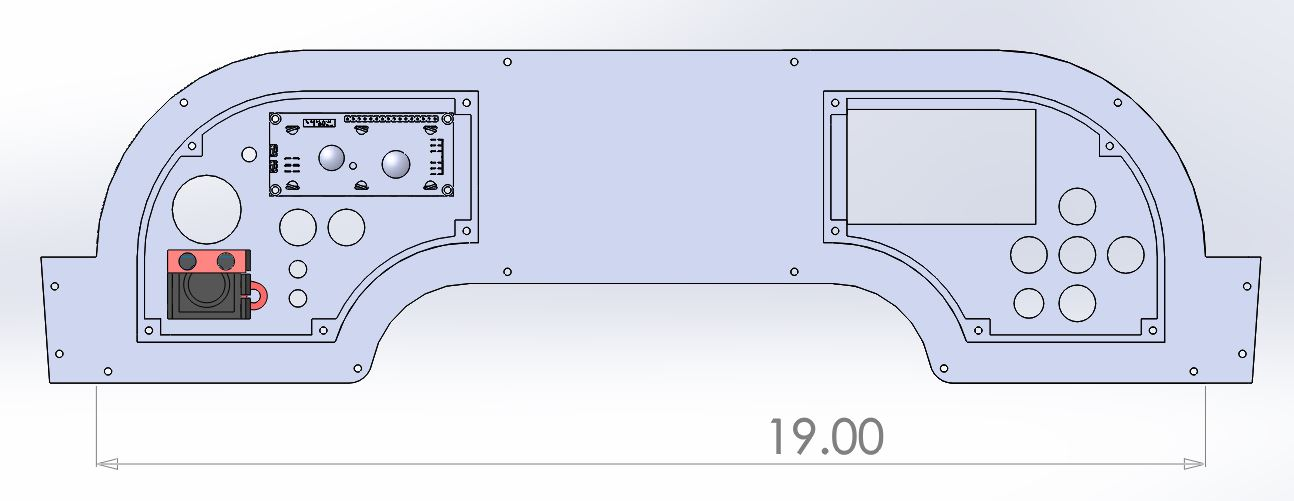
\includegraphics[width=\linewidth]{Dashboard_Rendering_Rear}
	\caption{Rendering of the dashboard module as seen from the back} \label{fig:Dashboard Render}
\end{figure}

For calculation of sound attenuation over distance, see \href{http://www.sengpielaudio.com/calculator-distance.htm}{SengpielAudio Distance Law Equation}
\end{document}
